\section{Tools} \label{sec:tools}

This section describes the tools used for the scrub process. 
With the requirement for agility, collaborative working and ease of linking to existing tools, Google Workspace is the chosen platform on which all the Rubin planning tools, including the scrub tool, have been developed. 
The particular tool that supports the annual scrub is a Google Sheets workbook called the ``Scrub Sandbox.''
It needs to facilitate:
\begin{enumerate}
\item capturing the current state of the operations plan for each team;
\item capturing what the desired changes are;
\item inputting flow down milestones for the upcoming FY based on higher level milestones defined by the Directors Office;
\item standardizing inputs coming in from the Departments and Teams;
\item easiy visualization of the impact of the desired change on the labor and non-labor budgets;
\item collaboration between Team Leaders as they work through their competing needs.
\end{enumerate}

\begin{figure}[h!]
\begin{centering}
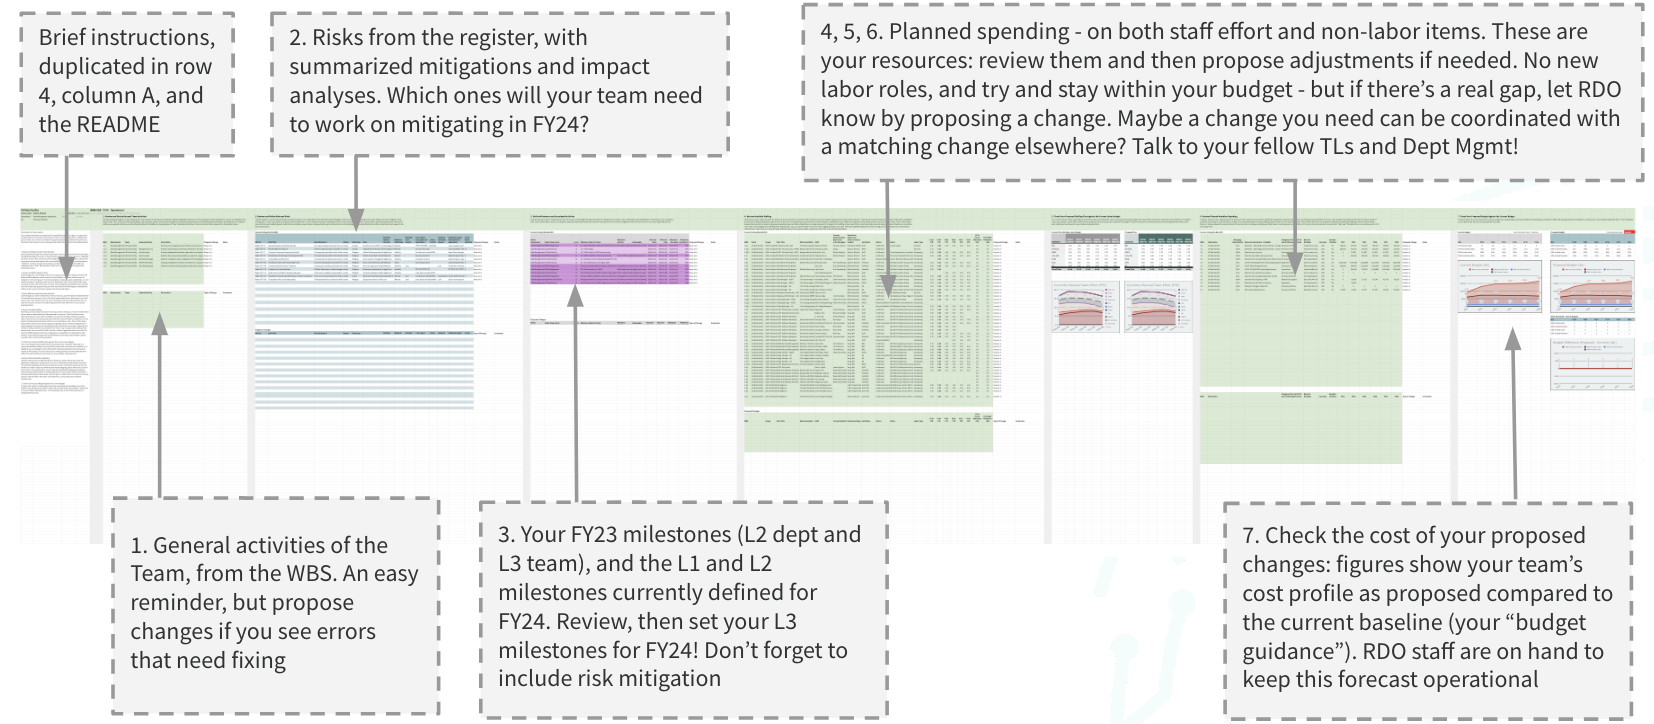
\includegraphics[width=1.0\textwidth]{Figure3OverviewScrubSandbox}
	\caption{ Overview of the Scrub Sandbox tool.
\label{fig:sandbox}}
\end{centering}
\end{figure}

\noindent Furthermore, the tool needs to enable the following aspects of the overall operations plan to be scrubbed:
\begin{enumerate}
\item Work Breakdown Structure (WBS);
\item risks;
\item Milestones;
\item Labor expenditure;
\item Non-labor expenditure.
\end{enumerate}
Each Team is provided with a sheet within the workbook, that follows a standard layout. 
The worksheet is organized into 7 vertical sections, where the left to right flow is through each of the aspects in the above list. 
Within all sections of all worksheets, the tool implements a standard approach to the proposing of changes (see \autoref{fig:wbs}).
An upper block of cells displays the current plan for that aspect, imported dynamically from the relevant planning tool using the \texttt{importrange} command (e.g. the vital information for the risks assigned to a team are read in from the Risk Register).
A lower block of cells is then available for proposed modifications to be entered.
A Proposed Change column is where any needed changes are flagged, chosen from the drop down choices which are Keep As-Is, Change, and Remove/Replace. 
There is space to enter a note if explanation is needed.
If either the value Change or Remove/Replace is chosen it will require a corresponding entry to be made in the Proposed Changes table lower block.

Proposed changes to the labor and non-labor plan are visualized in monetary terms in real-time with baseline comparison charts such as those shown in \autoref{fig:baseline}.



\begin{figure}[h!]
\begin{centering}
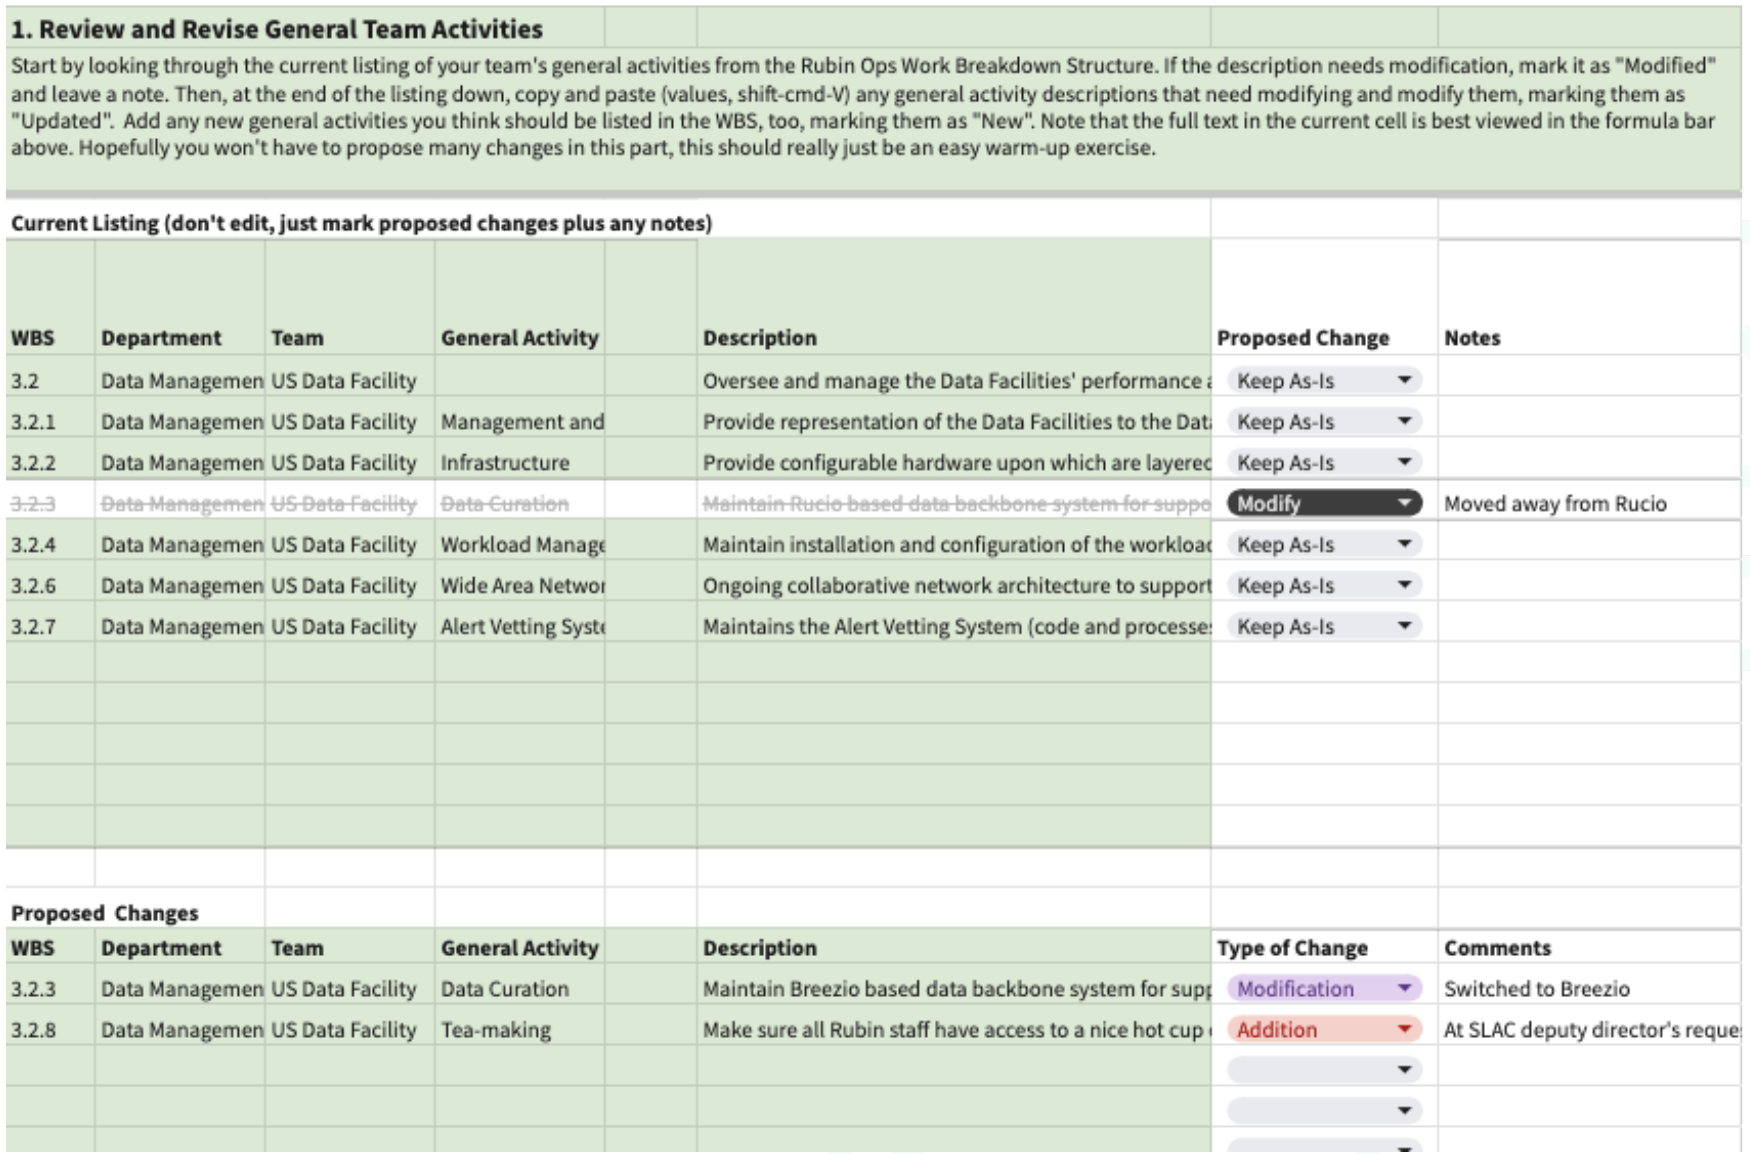
\includegraphics[width=1.0\textwidth]{Figure4WorkBreakdownStructurescrubbing}
	\caption{ Work Breakdown Structure scrubbing
\label{fig:wbs}}
\end{centering}
\end{figure}

\begin{figure}[hb!]
\begin{centering}
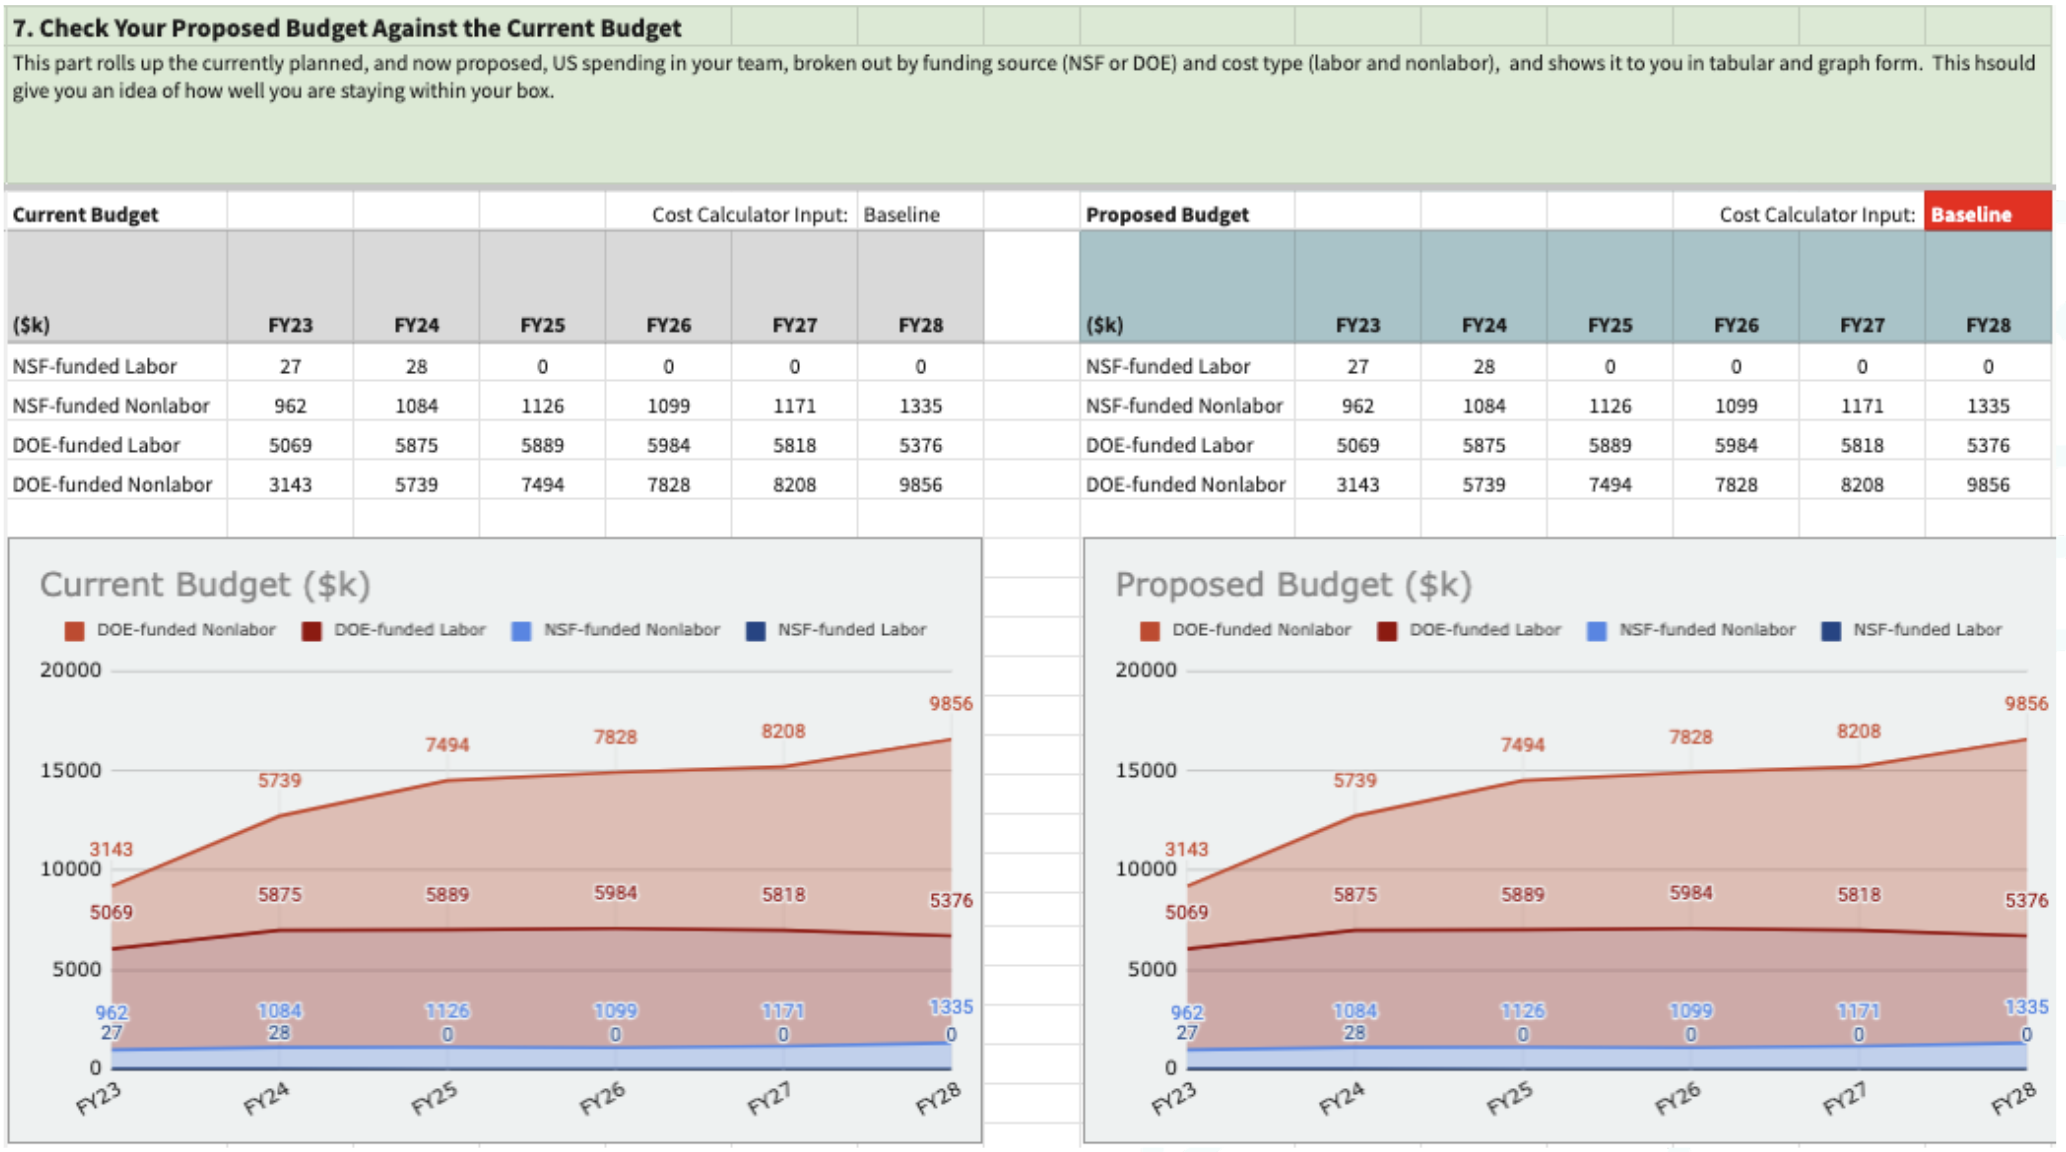
\includegraphics[width=1.0\textwidth]{Figure5BaselinevsProposed}
	\caption{Baseline vs Proposed labor and non-labor comparison
\label{fig:baseline}}
\end{centering}
\end{figure}
